\documentclass[10pt]{SelfArx} % Document font size and equations flushed left

\usepackage[english]{babel} % Specify a different language here - english by default

\usepackage[utf8]{inputenc} % Spanish tildes
\usepackage{epsfig} % for postscript graphics files
\usepackage{caption} % fig libraries
\usepackage{subcaption} % fig libraries

\usepackage{mathptmx} % math libraries
\usepackage{times} % math libraries
\usepackage{amsmath} % math libraries
\usepackage{amssymb} % math libraries
\usepackage{nccmath} % math libraries

\usepackage{siunitx} % SI symbols librarie


%----------------------------------------------------------------------------------------
%	COLUMNS
%----------------------------------------------------------------------------------------

\setlength{\columnsep}{0.55cm} % Distance between the two columns of text
\setlength{\fboxrule}{0.75pt} % Width of the border around the abstract

%----------------------------------------------------------------------------------------
%	COLORS
%----------------------------------------------------------------------------------------

\definecolor{color1}{RGB}{0,0,90} % Color of the article title and sections
\definecolor{color2}{RGB}{0,20,20} % Color of the boxes behind the abstract and headings

%----------------------------------------------------------------------------------------
%	HYPERLINKS
%----------------------------------------------------------------------------------------

\usepackage{hyperref} % Required for hyperlinks
\hypersetup{hidelinks,colorlinks,breaklinks=true,urlcolor=color2,citecolor=color1,linkcolor=color1,bookmarksopen=false,pdftitle={Title},pdfauthor={Author}}

%----------------------------------------------------------------------------------------
%	ARTICLE INFORMATION
%----------------------------------------------------------------------------------------

\JournalInfo{Fundamentals of Aerodynamics} % Journal information
\Archive{Laboratory report} % Additional notes (e.g. copyright, DOI, review/research article)


\PaperTitle{Wind Tunnel Data Acquisition and Analysis} % Article title


\Authors{Pablo Rodríguez Robles\textsuperscript{1}*\textsuperscript{\textdagger}} % Authors
\affiliation{\textsuperscript{1}\textit{University of León, León, Spain}} % Author affiliation
\affiliation{*\textbf{Corresponding author}: prodrr05@estudiantes.unileon.es} % Corresponding author
\affiliation{\textsuperscript{\textdagger}The Python code used to carry out the data analysis is available at: \url{https://github.com/PabloRdrRbl/aerodynamics_practrice}}

\Keywords{} % Keywords - if you don't want any simply remove all the text between the curly brackets
\newcommand{\keywordname}{Keywords} % Defines the keywords heading name

%----------------------------------------------------------------------------------------
%	ABSTRACT
%----------------------------------------------------------------------------------------

\Abstract{

The data from the wind tunnel allows us to obtain some fundamental aerodynamic characteristic of the NACA 0018 airfoil. Throughout this report the pressure distribution over the airfoil surface will be analyzed at different angles of attack in order to get the relationship between its lift coefficient and the angle of attack, after that we could obtain the lift produced by the airfoil or a scaled real wing (thanks to the non-dimensional analysis). Additionally, tunnel data are compared with the numerical ones provided by the popular software tool Xfoil, thus is possible to carry out a comparison between the numerical model and the wind tunnel data.
 
}

%----------------------------------------------------------------------------------------

\begin{document}

\flushbottom % Makes all text pages the same height

\maketitle % Print the title and abstract box
\tableofcontents % Print the contents section

\thispagestyle{empty} % Removes page numbering from the first page

%----------------------------------------------------------------------------------------
%	ARTICLE CONTENTS
%----------------------------------------------------------------------------------------

\section*{Introduction} % The \section*{} command stops section numbering

\addcontentsline{toc}{section}{Introduction} % Adds this section to the table of contents

This experiment puts in practice the knowledge acquired after the study of the thin airfoil theory for symmetric airfoils. To that end, we have a NACA 0018 airfoil inside the tunnel, for which the limit of its span is the tunnel's walls (recreating the infinite span condition).

What we do is measure the pressure distribution over the upper and lower surfaces of the airfoil. When the airfoil is subject to the subsonic freestream flow, the flow velocity is altered by the presence of the airfoil, which, applying the Bernoulli equation to the flow streamlines increases the pressure distribution in relation to the pressure on the freestream. After calculating the pressure coefficient for both surfaces the area between the curves correspond to the normal force coefficient on the airfoil, and therefore the lift coefficient is easy to work out.

%------------------------------------------------

\section{Methodology of the experiment}

Once we have agreed that our target in the wind tunnel is obtaining the pressure distribution on the airfoil, that is to say, the pressure on different points along it, we must raise how to do this.

For this porpoise, the experimental setup consists of an airfoil with 37 pressure taps at its mid-span, which allows us to get the pressure on each of the points where the pressure taps are located. Apart from that we install a pitot probe, which provide us with the freestream pressure and the pressure at the stagnation point. All this samples are connected using tygon tubes and a selector to a transducer. In it we connect two port each time: the stagnation pressure (fixed, because it is the reference pressure for the calculation of pressure differences) and the airfoil pressure taps or the freestream port (which we change using the selector to get the measurement of each point).
The transducer provides the transformation of pressure differences between the two ports in a voltage which we can measure using a voltmeter. With the selector we repeat this procedure for all the points on the airfoil at $0^{o}, 7^{o}, 14^{o}$ and $21^{o}$ of angle of attack.

\begin{figure}[!h]
\centering
  \begin{subfigure}[b]{0.2\textwidth}
  \centering
    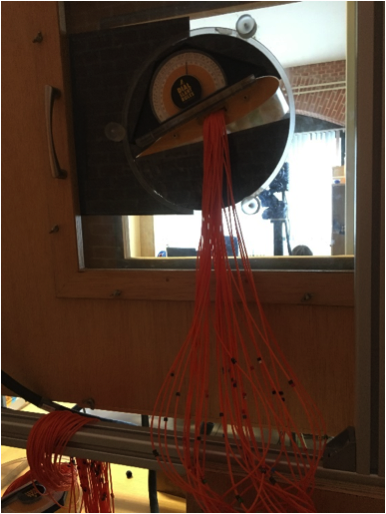
\includegraphics[scale=0.55]{photos/tunnel_setup_1}
    \caption{The airfoil has 37 pressure taps, which allows us to get the pressure.}
    \label{fig:f1}
  \end{subfigure}
  \hfill
  \begin{subfigure}[b]{0.2\textwidth}
  \centering
    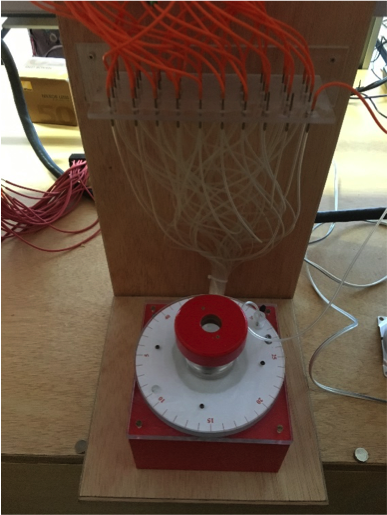
\includegraphics[scale=0.55]{photos/tunnel_setup_2}
    \caption{Using the selector we can choose the point where we measure.}
    \label{fig:f2}
  \end{subfigure}
  \caption{Laboratory setup.}
\end{figure}

%------------------------------------------------

\section{Data analysis}

\subsection{Analysis of the experimental voltages and calculation of the pressure coefficients}

As explained above, the data obtained in the wind tunnel is the voltage that the transducer returns. Since we want pressure differences, we must process our data.

Let us remember that our lab setup measures differences of pressures between the reference pressure (stagnation pressure) and the selected point. In this way, the relationship between the voltage and the pressure is linear and follows the expression shown below: 

\begin{equation} p_{i} - p_{\infty} = k (volts - offset) \end{equation}

Given that we are going to effectuate the non-dimensionalisation of the problem, it will not be necessary to know the constant which relates both magnitudes. By dividing the pressure differences it does not take action. In order to compute the pressure coefficient ($C_{p}$) on each of the points of the airfoil we assume that his equation is: 

\begin{equation} C_{p} = \frac{p_{i} - p_{\infty}}{\frac{1}{2} \rho {U_{\infty}}^{2}} \end{equation}

Note that the denominator of (2) is que stagnation pressure of the freestream, which we get from the pitot probe in the form of difference between it and the freestream pressure when we measure in the 40 port. Hence:

\begin{equation} C_{p} = \frac{p_{i} - p_{\infty}}{p_{s} - p_{\infty}} = \frac{p_{i} - p_{s} + p{s} - p_{\infty}}{p_{s} - p_{\infty}} = 1 - \frac{p_{i} - p_{s}}{p_{s} - p_{\infty}} \end{equation}


Combining (1) and (3) we have that for each point $i$:

\begin{equation} C_{p} = 1 - \frac{k (volts - offset)_{i}}{k (volts - offset)_{40}} \end{equation}
 
It is important to keep in mind the offset correction. The ofsset exist because of the lack of the transducer calibration. We know that the stagnation point is located at the place were $C_{p} = 1$, condition that based on (4) will be satisfied when the voltage (pressure difference at its core) is zero. Thus, this must be the lowest value (there is no pressure coefficient greater than 1) and if we do not correct it there will not be stagnation point.

Personally, I have subtracted the minimum voltage obtained to the whole dataset for each angle of attack, so it will be always a voltage equal to zero.

Following this procedure for all the angles of attack we can plot the pressure coefficients along the airfoil at each of them.

\begin{figure}[ht!]
\centering
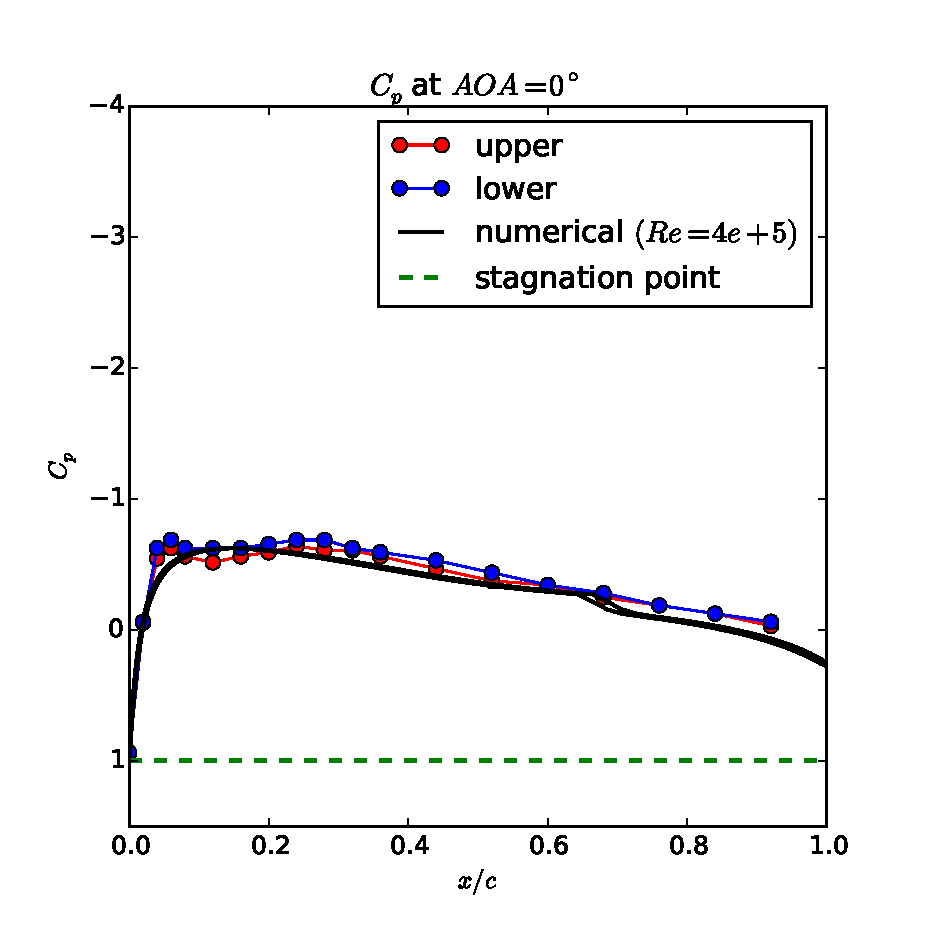
\includegraphics[scale=0.55]{plots/compared-cp-at-aoa0.eps} 
\caption{Pressure coefficient along the NACA 0018 airfoil at $0^{o}$ angle of attack. Experiment vs. numerical solution. }
\end{figure}

\begin{figure}[ht!]
\centering
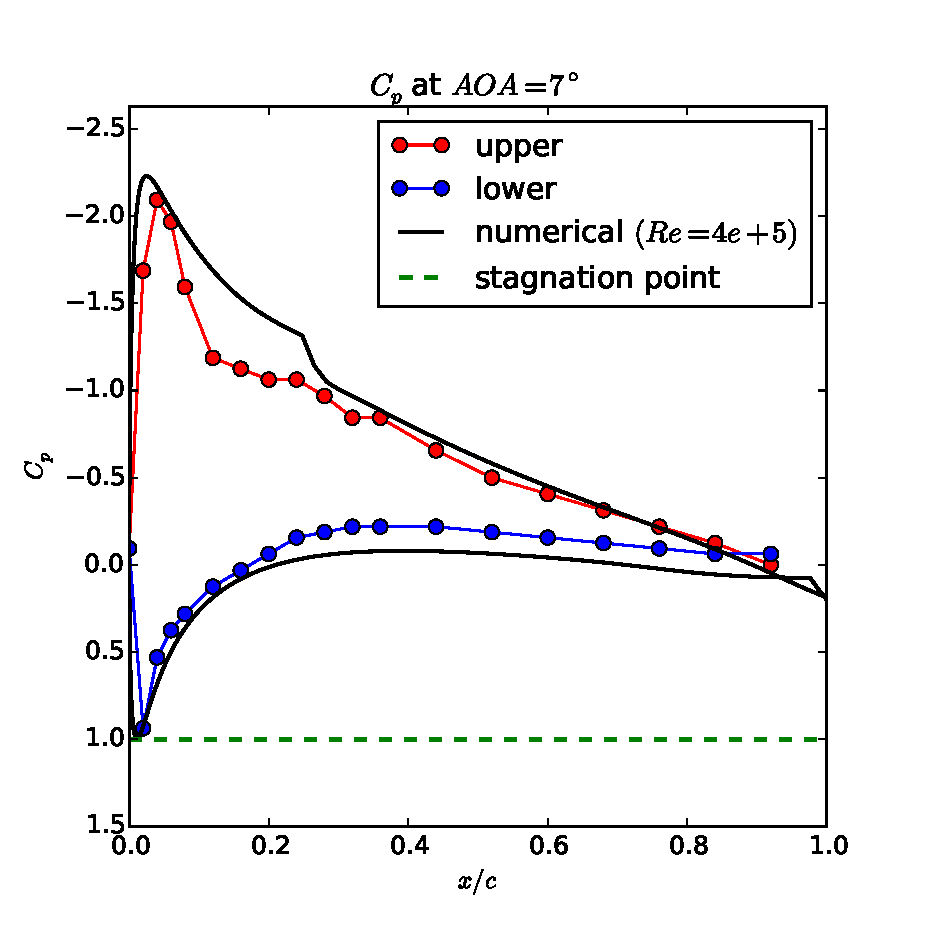
\includegraphics[scale=0.55]{plots/compared-cp-at-aoa7.eps}
\caption{Pressure coefficient along the NACA 0018 airfoil at $7^{o}$ angle of attack. Experiment vs. numerical solution.}
\end{figure}

\begin{figure}[ht!]
\centering
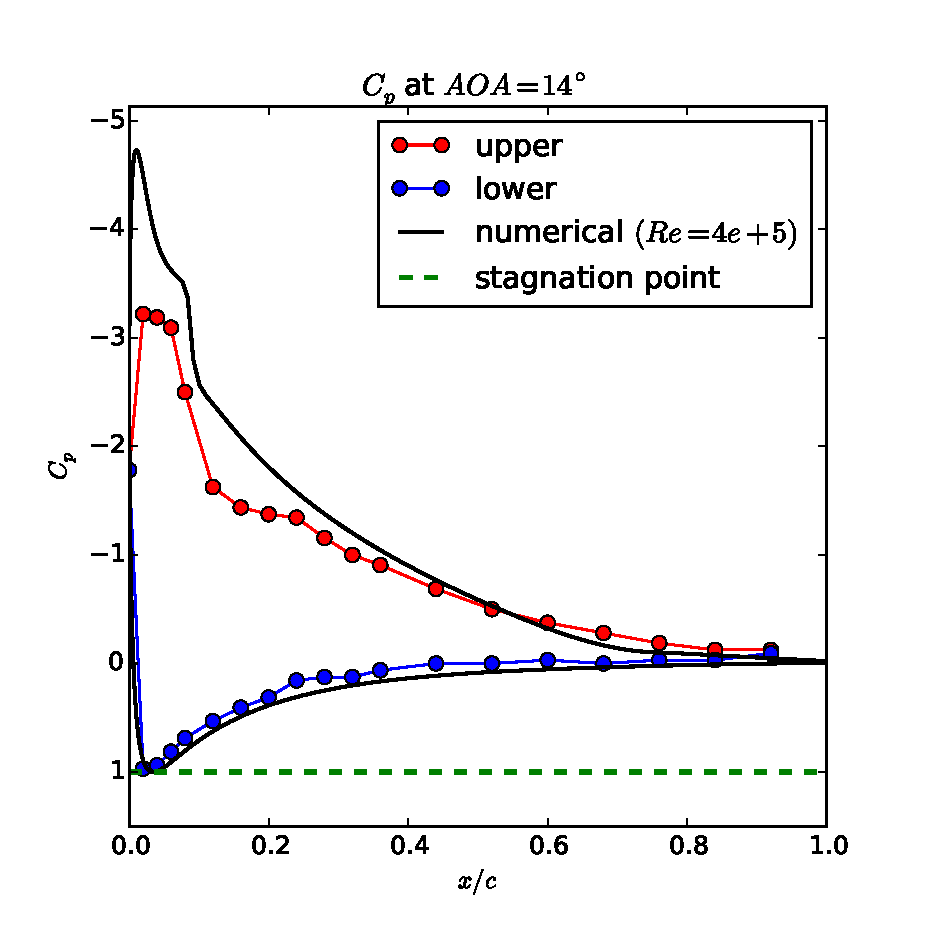
\includegraphics[scale=0.55]{plots/compared-cp-at-aoa14.eps}
\caption{Pressure coefficient along the NACA 0018 airfoil at $14^{o}$ angle of attack. Experiment vs. numerical solution.}
\end{figure}

\begin{figure}[ht!]
\centering
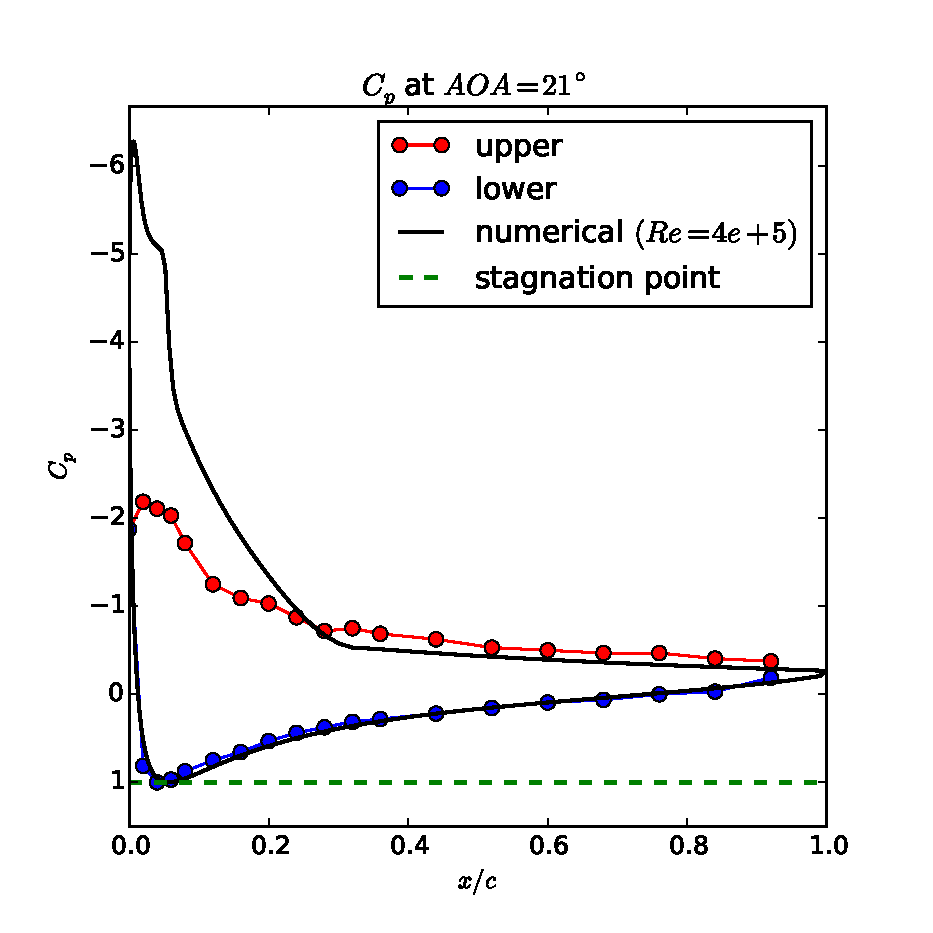
\includegraphics[scale=0.55]{plots/compared-cp-at-aoa21.eps}
\caption{Pressure coefficient along the NACA 0018 airfoil at $21^{o}$ angle of attack. Experiment vs. numerical solution.}
\end{figure}

As can be seen in the figures, a comparative with a numerical solution is represented, in addition to experimental pressure coefficients. The software tool used to get it is a Python script \cite{Pablo:source-code} which calls Xfoil \cite{Drela:user-primer}, that gets the commands needed to numerically solve the problem with the conditions imposed. This comparative will be commented further on.

\subsection{Calculation of the lift coefficient}

Once we get the airfoil's pressure coefficients at the four angles of attack, we proceed to compute the lift coefficient. We find that it is given by the following expression \cite{Anderson:book-fundamentals}:

\begin{equation} c_{l} = c_{n} \cos{\alpha} - c_{a} \sin{\alpha} \end{equation}

Where:

\begin{eqnarray}\nonumber
c_{n} & = & \frac{1}{c} \left[ \int_{0}^{c} (C_{p, l} - C_{p,u}) dx \hspace{0.2cm} + \right.\\
& & \hspace{0.3cm} \left. \int_{0}^{c} (c_{f, u}\frac{dy_u}{dx}  + c_{f,l}\frac{dy_l}{dx}) dx \right]
\end{eqnarray}

\begin{eqnarray}\nonumber
c_{a} & = & \frac{1}{c} \left [  \int_{0}^{c} (C_{p, u}\frac{dy_u}{dx}  - C_{p,l}\frac{dy_l}{dx}) dx \hspace{0.2cm} + \right.\\  
& & \hspace{0.3cm} \left. \int_{0}^{c} (c_{f, u} + c_{f,l}) dx  \right] \end{eqnarray}

For the sake of simplicity, we will use and expression which does not involve the friction forces ($c_f$), nor will we work in the equation (7) with the airfoil's geometry. When we approach to the integral (6) we should realize that we are not using the real distance between the pressure taps on the airfoil, but we consider distance over the airfoil's chord. Thus our target integral will not have the $\frac{1}{c}$ with which equation (6) starts and its integration limits will be from 0 to 1. So:

\begin{equation} c_{l} = c_{n} \cos{\alpha} \end{equation}

\begin{equation} c_{n} = \int_{0}^{1} (C_{p, l} - C_{p,u}) d(x/c)\end{equation}

The following step is solve the integral (9), for this we will use a numerical integration method. The easiest one is the trapezoidal rule for a non-uniform grid:

\begin{equation} C_{p,u}, C_{p,l} = \sum_{i  =1}^{n-1} \frac{C_{p,i} + C_{p,i+1}}{2} (x_{i + 1} - x_{i}) \end{equation}

Where $i$ are the pressure taps on each surface and $n$ the sum of them.

\begin{figure}[ht!]
\centering
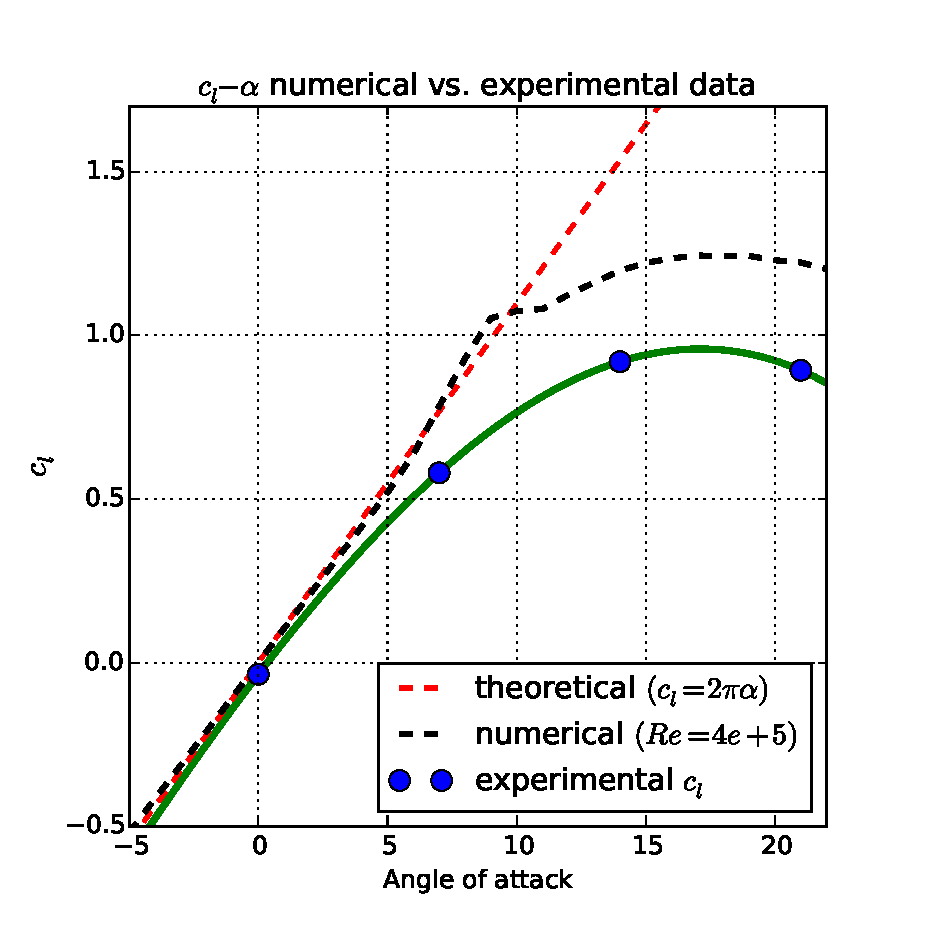
\includegraphics[scale=0.55]{plots/cl-alpha.eps}
\caption{Lift coefficient computation per unit of span for different angles of attack. Experiment vs. numerical solution vs. theory.}
\end{figure}

\newpage

%------------------------------------------------

\section{Data discussion}
\subsection{Pressure coefficient values}

As stated above, the pressure coefficient plots are accompanied with the numerical solution obtained using Xfoil. When we try to get this computational solution we need to set the Reynolds number of the wind tunnel:

\begin{equation} Re = \frac{inertial forces}{viscous forces}  = \frac{\rho U_{\infty} L}{\mu} \end{equation}

Assuming ISA conditions at the altitude of León ($\SI{837}{\meter}$), knowing that the airfoil's chord is $c = \SI{0.25}{\meter}$ and measuring the freestream velocity using the pitot probe (port number 40), we get a Reynolds number of the order of magnitude of $Re = \num{3.7e4}$. The problem is that Xfoil does not converge at a low Reynolds number such as this \cite{Drela:low-reynolds}, so it has been necessary to increase its magnitude to make it happen. 

Note that at the two first angles of attack the experimental values are very close to the Xfoil ones. As we can see in the $c_l - \alpha$ plot, the airfoil stalls near to $14^{o}$. When the boundary layer separation is greater ($21^{o}$) the pressure coefficient increases, in other words, pressure increases at the upper surface due to the boundary layer separation.

Perhaps, because of the computational Reynolds number is greater that in the wind tunnel, the $C_p$ prediction is lower, flow separation in the tunnel leads to the increase of the pressure. (See that the y-axis is inverted in the plots, so lower is greater in them). 

The separation of flow from the upper wing surface at high angles of attack is quite different at low Reynolds number from that at the high Reynolds numbers of real aircraft. High-pressure wind tunnels are one solution to this problem \cite{Anderson:book-history}.

If the Xfoil code converged, we could see that the experimental data are pretty close to them, and distant to the theory given the low Reynolds number.

\subsection{Lift coefficient values}

In spite of the problems due to the differences with the Reynolds number and the flow separation, it can be said that the $c_l - \alpha$ curve obtained is quite consistent.
Firstly, we can see a linear region, which is not very closes to $2\pi$ (thin airfoil theory), neither to the numerical values. This is mostly because of the flow separation, but also because of the measuring errors. As can be seen, the numerical solution is close to the theoretical value.

At low Reynolds numbers the upper boundary layer detaches from the airfoil even with low angles of attack. At low Reynolds numbers but above $Re = \num{3e4}$ \cite{Gerakopulos:naca-low} (fairly similar to the estimated wind tunnel $Re$) the turbulent flow reattaches, but below it does not, leading to the comment decrease of the upper pressure.

Before the lineal region can be found that there is a maximum value of the lift coefficient ($c_{lmax}$) followed by the decrease of it (stall), that is the expected behavior.

Net lift does not happen at zero angle of attack because of the symmetrical airfoil used in the experiment.

\subsection{Other errors}

Finally, in addition to the previous analysis, there are other factors which could lead to the data deviation. Some of them are:

\begin{itemize}

\item Wind tunnel wall interference effects due to proximity exists near the walls of the tunnel, what leads to inaccuracies in the measure of the pitot probe, placed near these walls. Moreover, it could affect the airfoil surface, so that pressure measurements could not be extrapolated to free-fligth conditions. In order to cope with this problem we could introduce some corrections in the instruments or model the wall interference phenomena in our code \cite{Duraisamy:wall-interference}.

\item As stated above, pressure loses in the tunnel or along the tubes could affect the data.

\item The precision of the instrument used to read the pressure of each point (voltmeter) is not high enough to get precise data. 

\item The reading of the number given by the voltmeter depends on the person who is reading it, furthermore the voltmeter is continuously oscillating. 

\item As the pressure is converted into electricity, some heat is lost, transforming the data.

\end{itemize}

%----------------------------------------------------------------------------------------
%	REFERENCE LIST
%----------------------------------------------------------------------------------------

\phantomsection
\bibliographystyle{unsrt}
\bibliography{references}

%----------------------------------------------------------------------------------------

%----------------------------------------------------------------------------------------

\begin{figure*}[!ht]
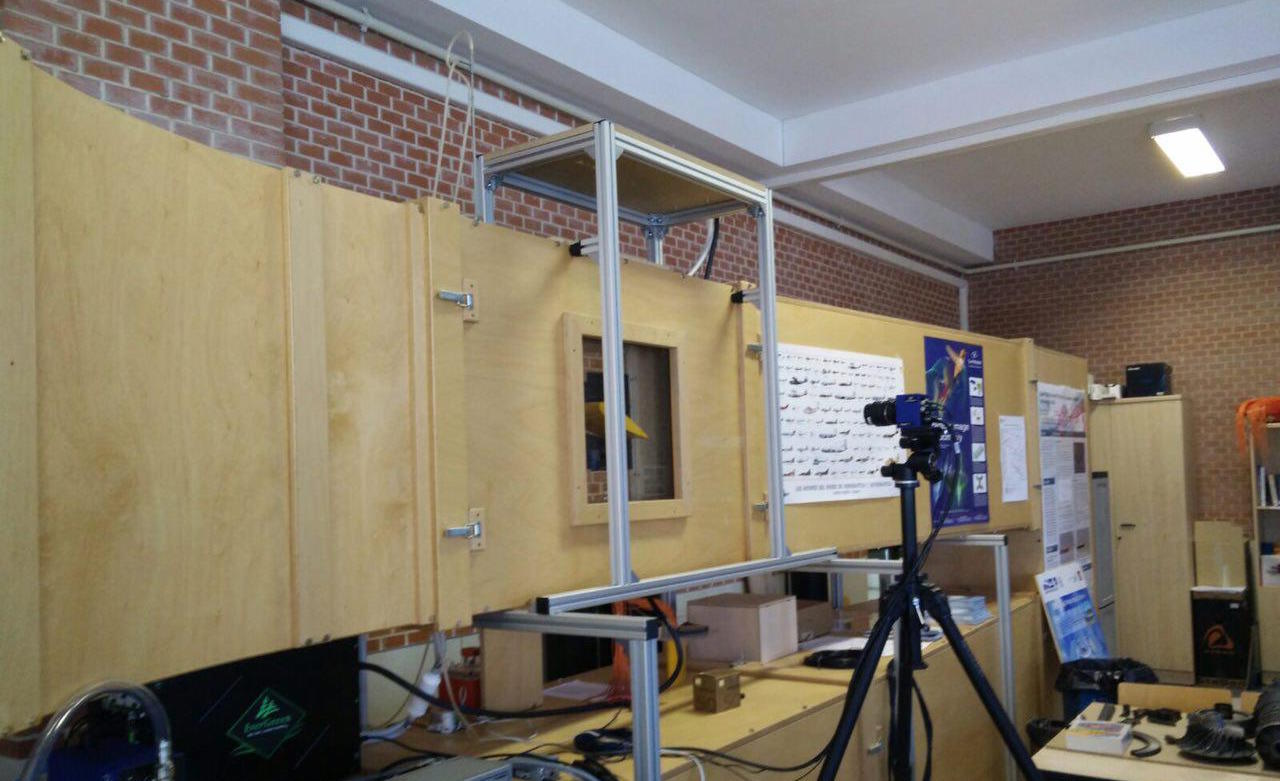
\includegraphics[width=\linewidth]{photos/tunnel_setup_3} 
\caption{Wind tunnel lab setup. On top of the tunnel we can see the pitot probe with the static tab and the stagnation pressure one.}
\end{figure*}


\end{document}